\documentclass[10pt]{article}
\usepackage[utf8]{inputenc}
\usepackage{listings}
\usepackage{float}
\usepackage{graphicx}
\usepackage{fullpage}
\usepackage{caption}
\usepackage{subcaption}
\usepackage{amsmath}

%\renewcommand{\thesubsection}{\arabic{subsection}}
\renewcommand{\thesubsubsection}{\alph{subsubsection}}

\title{Pattern Recognition Practical 3}
\author{Group 24: \and Maikel Withagen (s1867733) \and Steven Bosch (s1861948)}
\date{\today}
\lstset{
frame=single, 
numbers=left, 
breaklines=true, 
language=Matlab,
basicstyle=\small, 
title=\lstname
}

\renewcommand{\thesection}{Assignment \arabic{section}}
\renewcommand{\thesubsection}{\arabic{subsection}}
\begin{document}

\maketitle

\section{Classification error, hit/false alarm rates, ROC curve, discriminability}
\subsection{}
Figure \ref{fig1.1} shows the ROC-curves we acquired using the code given in the listing for assignment 1.1 in the appendix. The figure shows that the higher the difference between the means of the two distributions is (i.e. the further away the distributions are from each other), the higher the number of hits is per number of fals alarms. This means that classification will go better when distributions are farther away from each other, which is of intuitively comprehensable as well.

\begin{figure}[H]
 \centering
 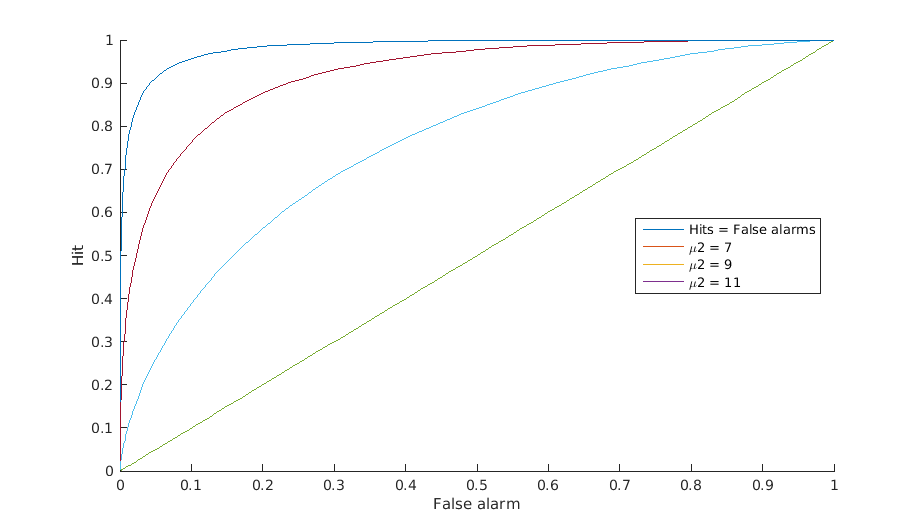
\includegraphics[width=\textwidth]{assign1_1.png}
 \caption{ROC-curves for $\mu_2={7, 9, 11}$ and the hits $=$ false alarms marker line.}
 \label{fig1.1}
\end{figure}

\subsection{}
Figure \ref{fig1.2} shows the point $(fa, h)$ of the two given binary vectors plotted in the plot computed in assignment 1.1. The listing for assignment 1.2 in the appendix gives the code used to compute this point and to compute the ROC-curve with the associated discriminability value $d'$. Trial and error yielded a ROC-curve with $d' \approx 1.5$ (this is an approximation, the exact value is a decimal value that is time-consuming to find by trial and error). We computed this using $\sigma_{1,2} = 1$, which yields $\mu_2-\mu_1 = 1.5$ for the found discriminability value. Note that the code in the listing gives $\sigma = 2$, which means $\mu_2-\mu_1 = 3$, since $d' = \frac{\mu_2-\mu_1}{\sigma}$. So as long as the discriminability valueb between two distributions is the same, the sigma does not matter for classification. 

\begin{figure}[H]
 \centering
 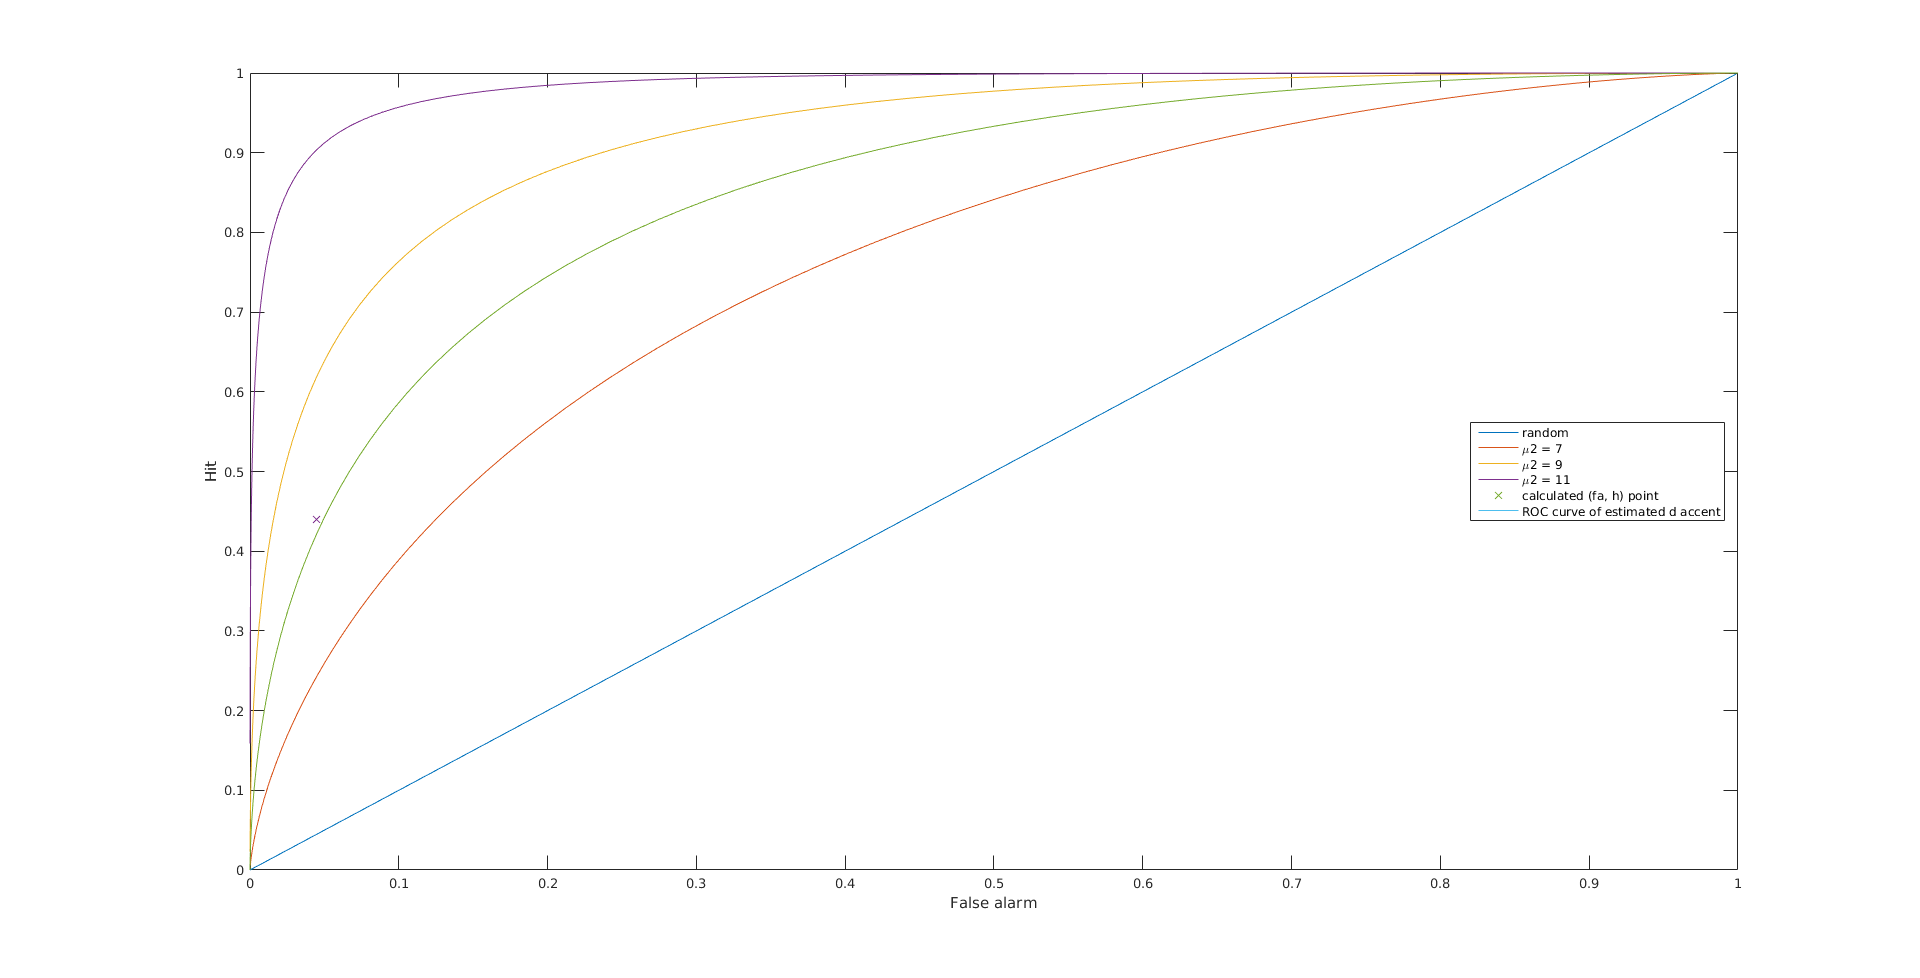
\includegraphics[width=\textwidth]{assign1_2b.png}
 \caption{Plot of the $(fa, h)$ point, the ROC-curves for $\mu_2={7, 9, 11}$, the hits $=$ false alarms marker line, and the ROC-curve with $d'=1.5$.}
 \label{fig1.2}
\end{figure}

\section{K-nearest neighbor classification}
\subsection{}
Our implementation of the KNN-function is the following:
\lstinputlisting{../Code/KNN.m}

\subsection{}
For $k={1, 3, 5, 7}$ this implementation yields the classification grid shown in figure \ref{fig2.1}:
\begin{figure}[H]
  \centering
  \begin{subfigure}{.48\textwidth}
    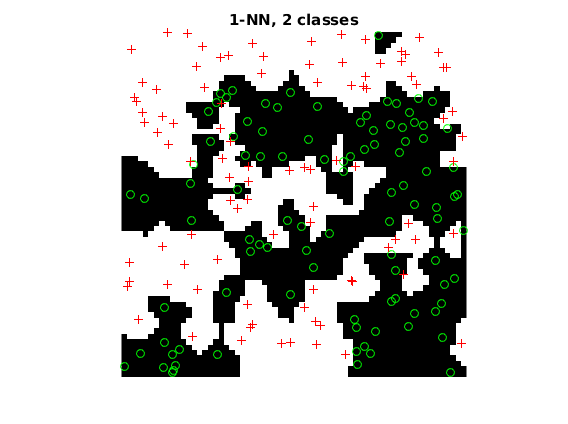
\includegraphics[width=1\linewidth]{assign2_2_1.png}
    \caption{Classification grid of the data set using KNN (for $k=1$)}
    \label{fig2.1a}
  \end{subfigure}
  \begin{subfigure}{.48\textwidth}
    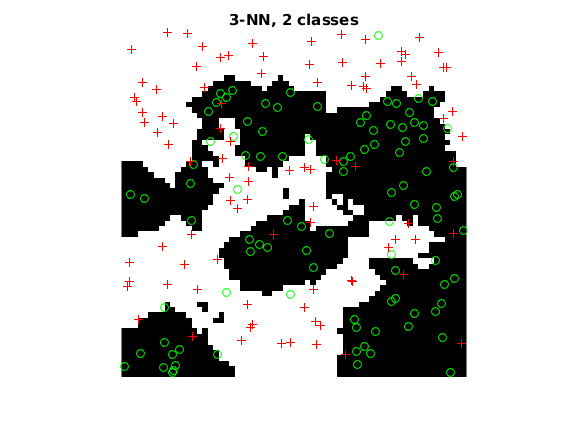
\includegraphics[width=1\linewidth]{assign2_2_3.png}
    \caption{Classification grid of the data set using KNN (for $k=3$)}
    \label{fig2.1b}
  \end{subfigure}
  \begin{subfigure}{.48\textwidth}
    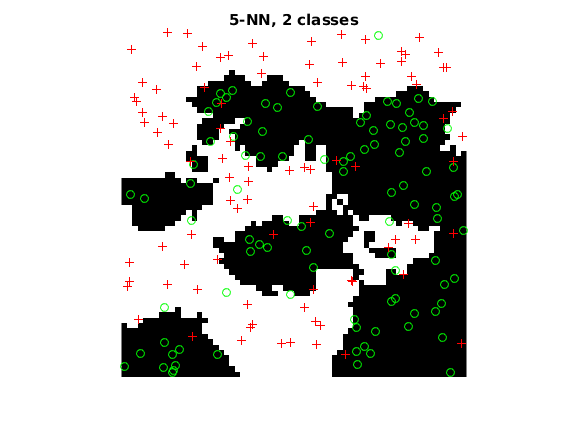
\includegraphics[width=1\textwidth]{assign2_2_5.png}
    \caption{Classification grid of the data set using KNN (for $k=5$)}
    \label{fig2.1c}
  \end{subfigure}
  \begin{subfigure}{.48\textwidth}
    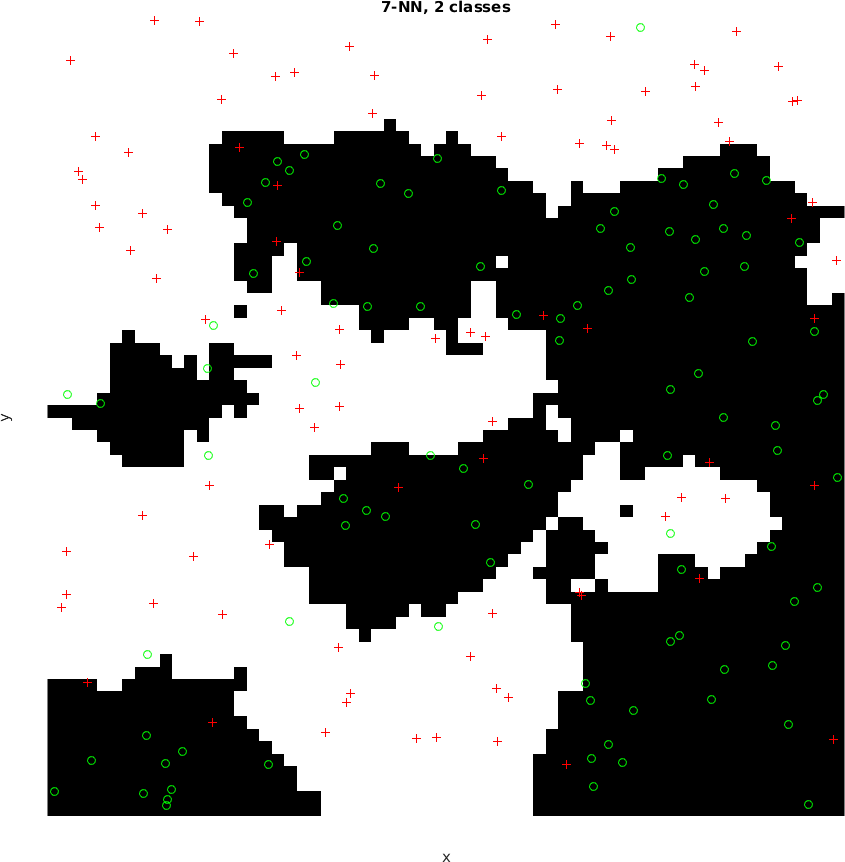
\includegraphics[width=1\textwidth]{assign2_2_7.png}
    \caption{Classification grid of the data set using KNN (for $k=7$)}
    \label{fig2.1d}
  \end{subfigure}
  \caption{Classification grids for different $k$s}
  \label{fig2.1}
\end{figure}

\subsection{}
Our implementation of the leave-one-out cross validation is given in the appendix. Figure \ref{fig2.3} gives the error rates we acquired for the diffferent values for $k$ using our implementation. The figure shows that a $k$ of 3 or 5 yields the best performance with an error rate of around 0.23. It is not illogical that the optimal $k$ is such a value. 

On the one hand a $k$ of 1 performs worse, because it does not account for outliers. With a $k$ of 1 outliers would classify a number of data points incorrectly, while increasing $k$ to 3 would already correct for that, because it is very unlikely that two outliers would be that close to each other that they would together misclassify a data point (you could even argue whether they would actually be outliers if they are close to each other). 

On the other hand when $k$ would become too high, data points are prone to be misclassified when they are closer to the decision boundary (for example when there are multiple points of the other class on the other side of the decision boundary which would be taken into account).

\begin{figure}[H]
 \centering
 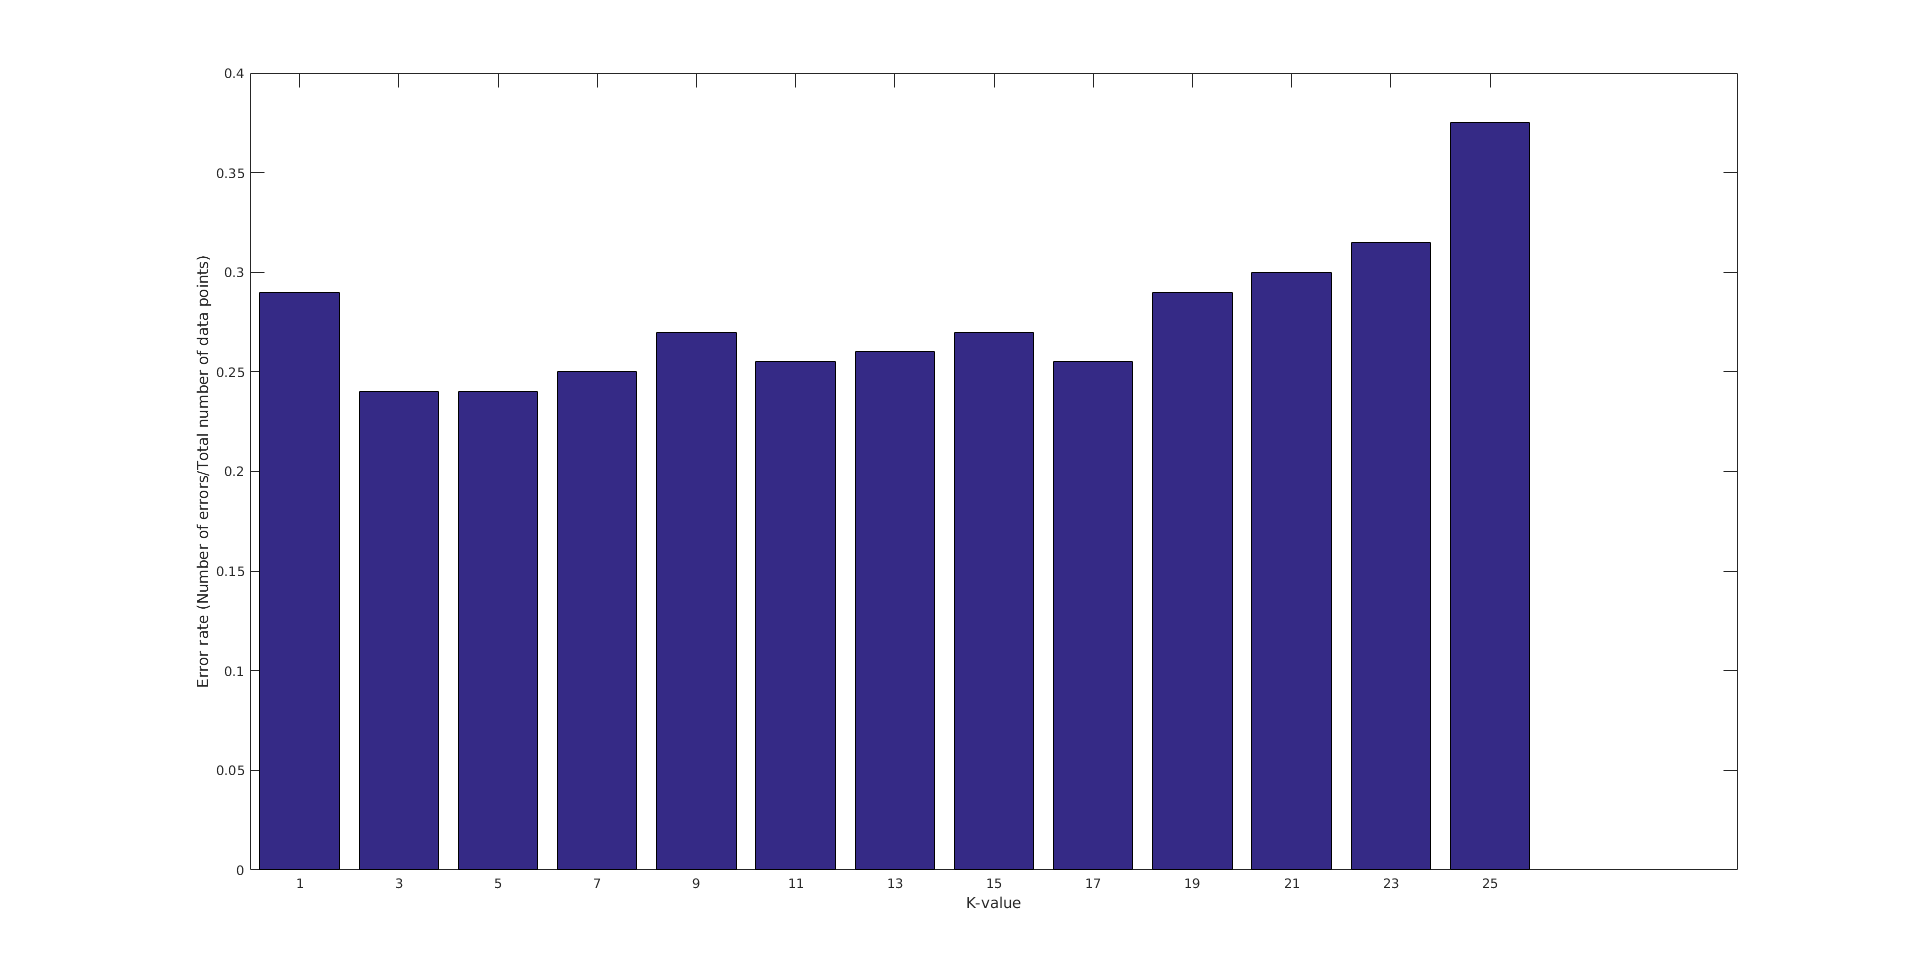
\includegraphics[width=\textwidth]{assign2_3.png}
 \caption{Error rate for different values of $k$ using leave-one-out cross validation.}
 \label{fig2.3}
\end{figure}

\subsection{}
To do classification for four classes we changed the parameter of classes to 4 and added the new classes to the plots. This resulted in the classification grids shown in figure \ref{fig2.4_a}. Cross validation with four classes yields the error rates given in figure \ref{fig2.4b}. The figures show that again most of the points get classified correctly. This time we find an optimum at only a k of 5 (not of 3 as well, as was the case with two classes). The average error rate does seem to be higher than with two classes though. This seems logical, because with random data you would expect that with more classes there is a higher probability of a data point being classified into the wrong class. This is however, totally dependent on the data. If the actual data represent four well divided classes, the classification would of course go better when you would actually use four classes, because when you would just use two, the data might be distributed over the two classes in such a way that there is not such a clear separation boundary as with four classes. 

In normal circumstances however, the classifier data would be seperated into logical groups instead of random groups like we do now. Then a difference in classifying performance would be logically explainable, because the data would actually represent groups already.

\begin{figure}[H]
  \centering
  \begin{subfigure}{.48\textwidth}
    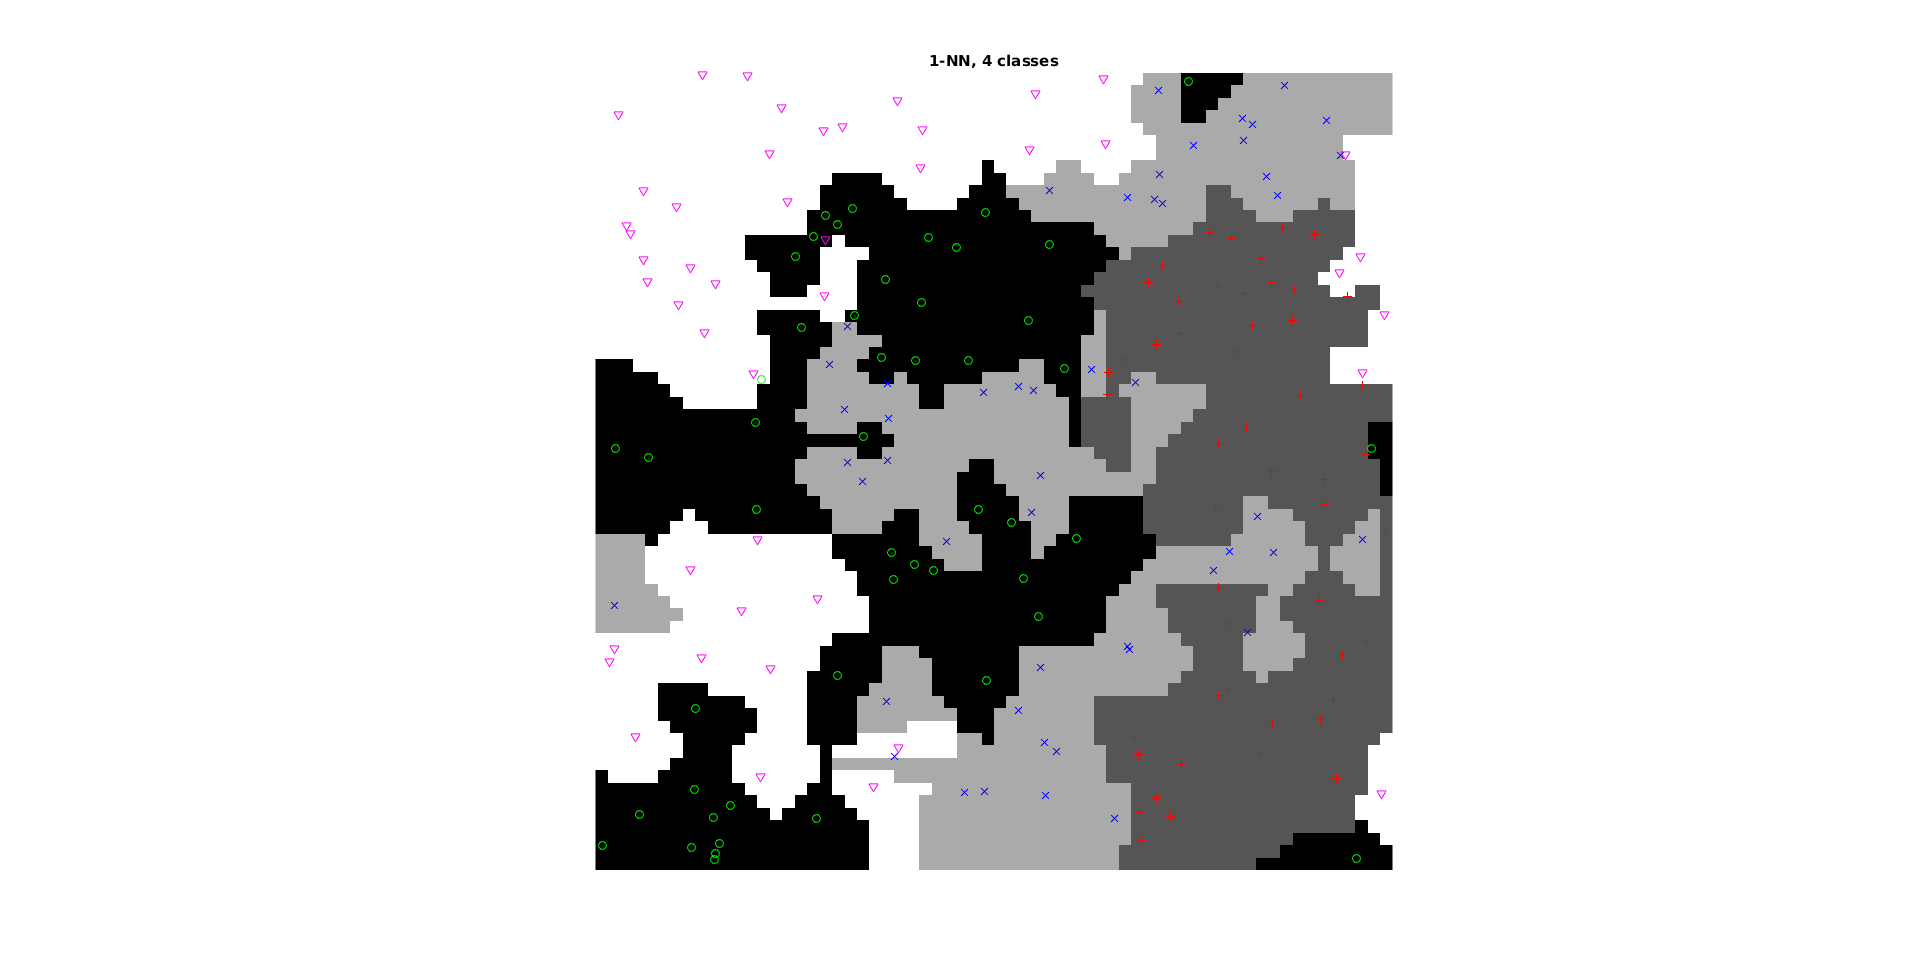
\includegraphics[width=.8\linewidth]{assign2_4_1.png}
    \caption{Classification grid of the data set using KNN (for $k=1$)}
    \label{fig2.4a}
  \end{subfigure}
  \begin{subfigure}{.48\textwidth}
    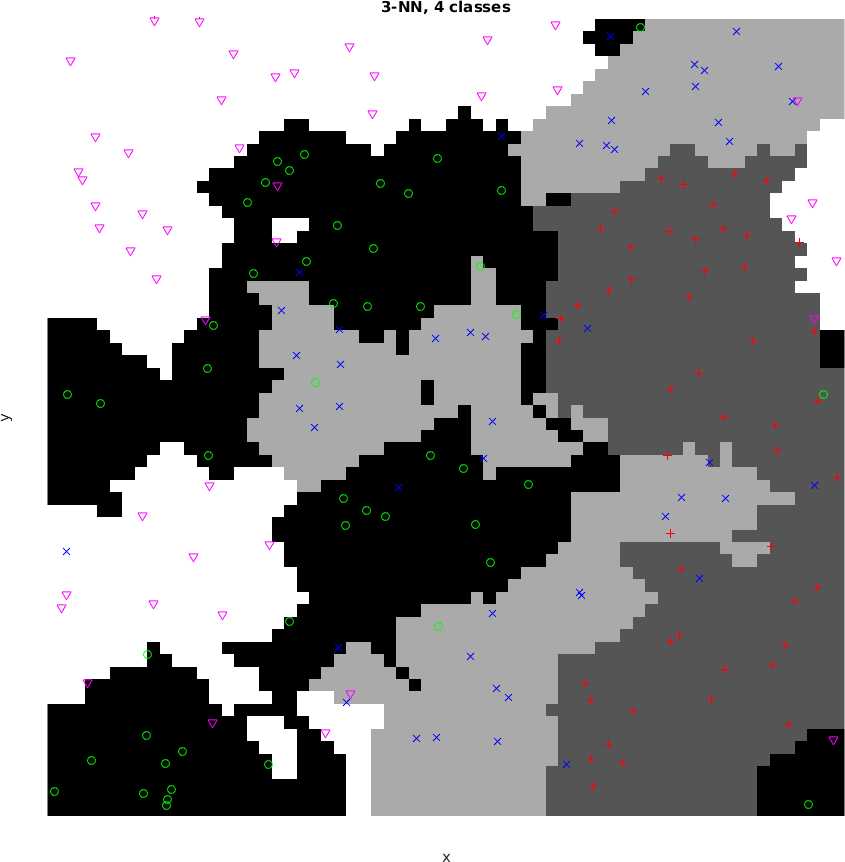
\includegraphics[width=.8\linewidth]{assign2_4_3.png}
    \caption{Classification grid of the data set using KNN (for $k=3$)}
    \label{fig2.4b}
  \end{subfigure}
  \begin{subfigure}{.48\textwidth}
    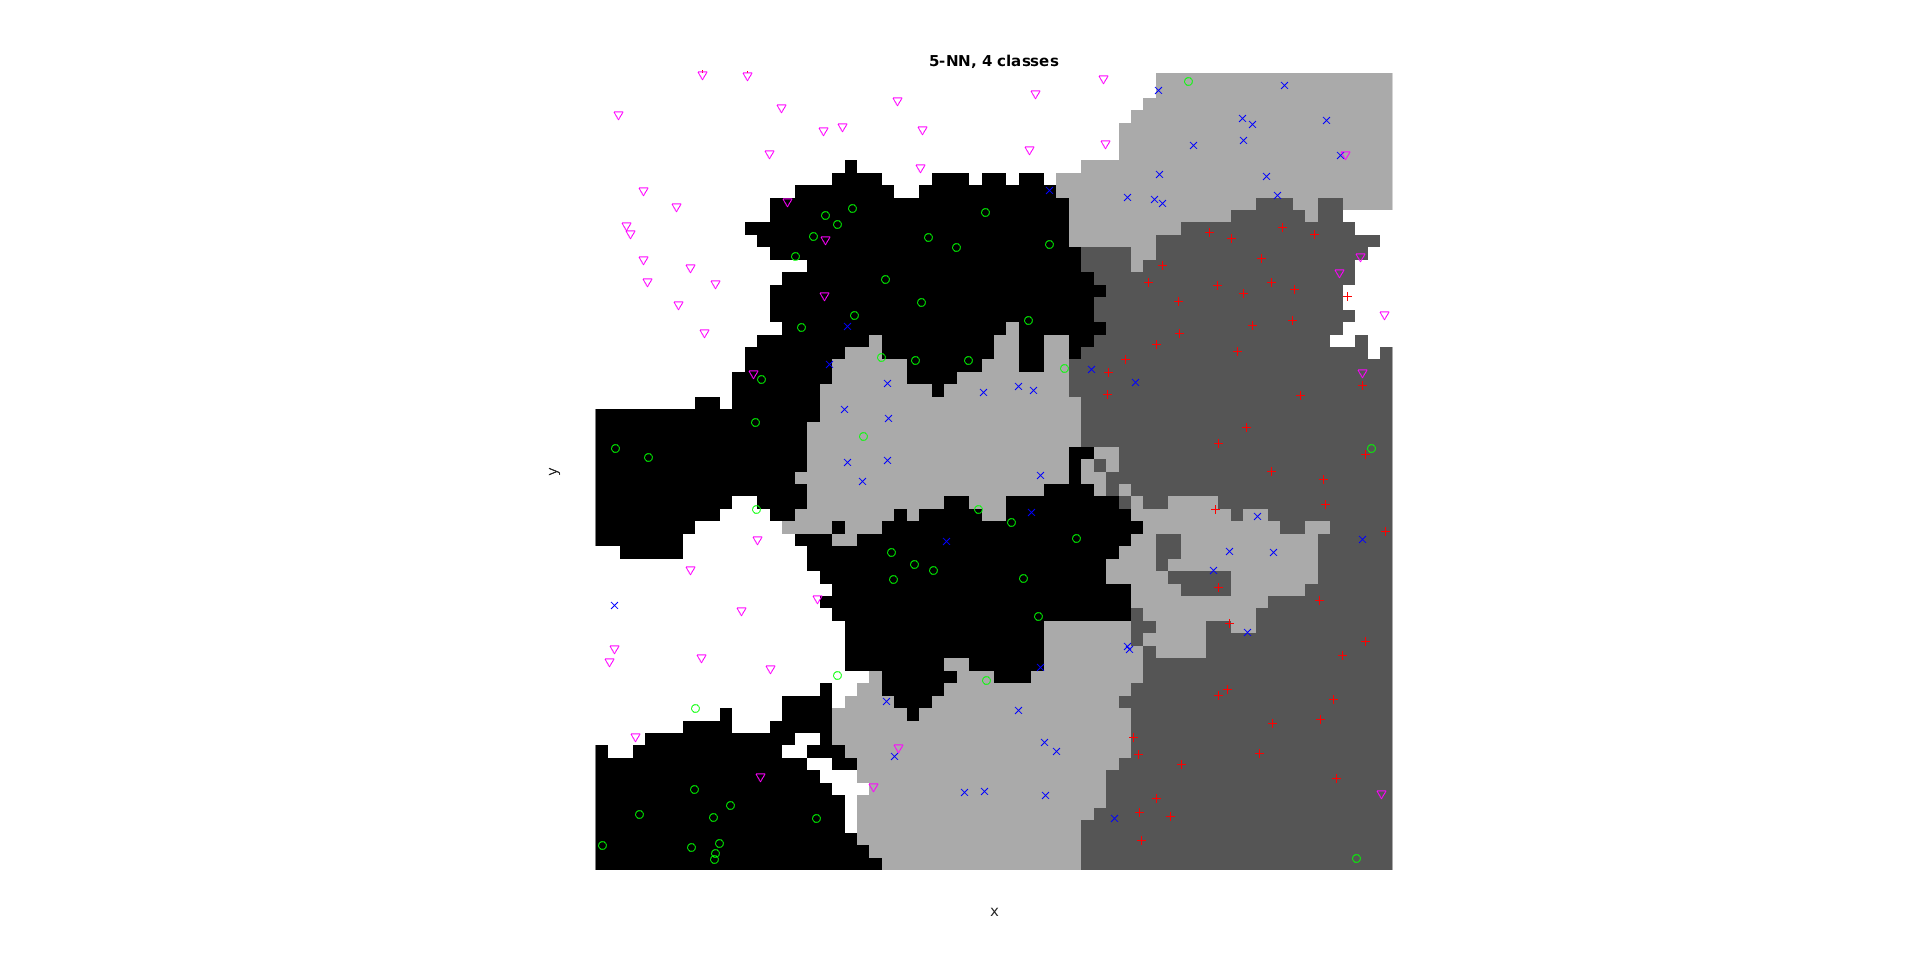
\includegraphics[width=.8\textwidth]{assign2_4_5.png}
    \caption{Classification grid of the data set using KNN (for $k=5$)}
    \label{fig2.4c}
  \end{subfigure}
  \begin{subfigure}{.48\textwidth}
    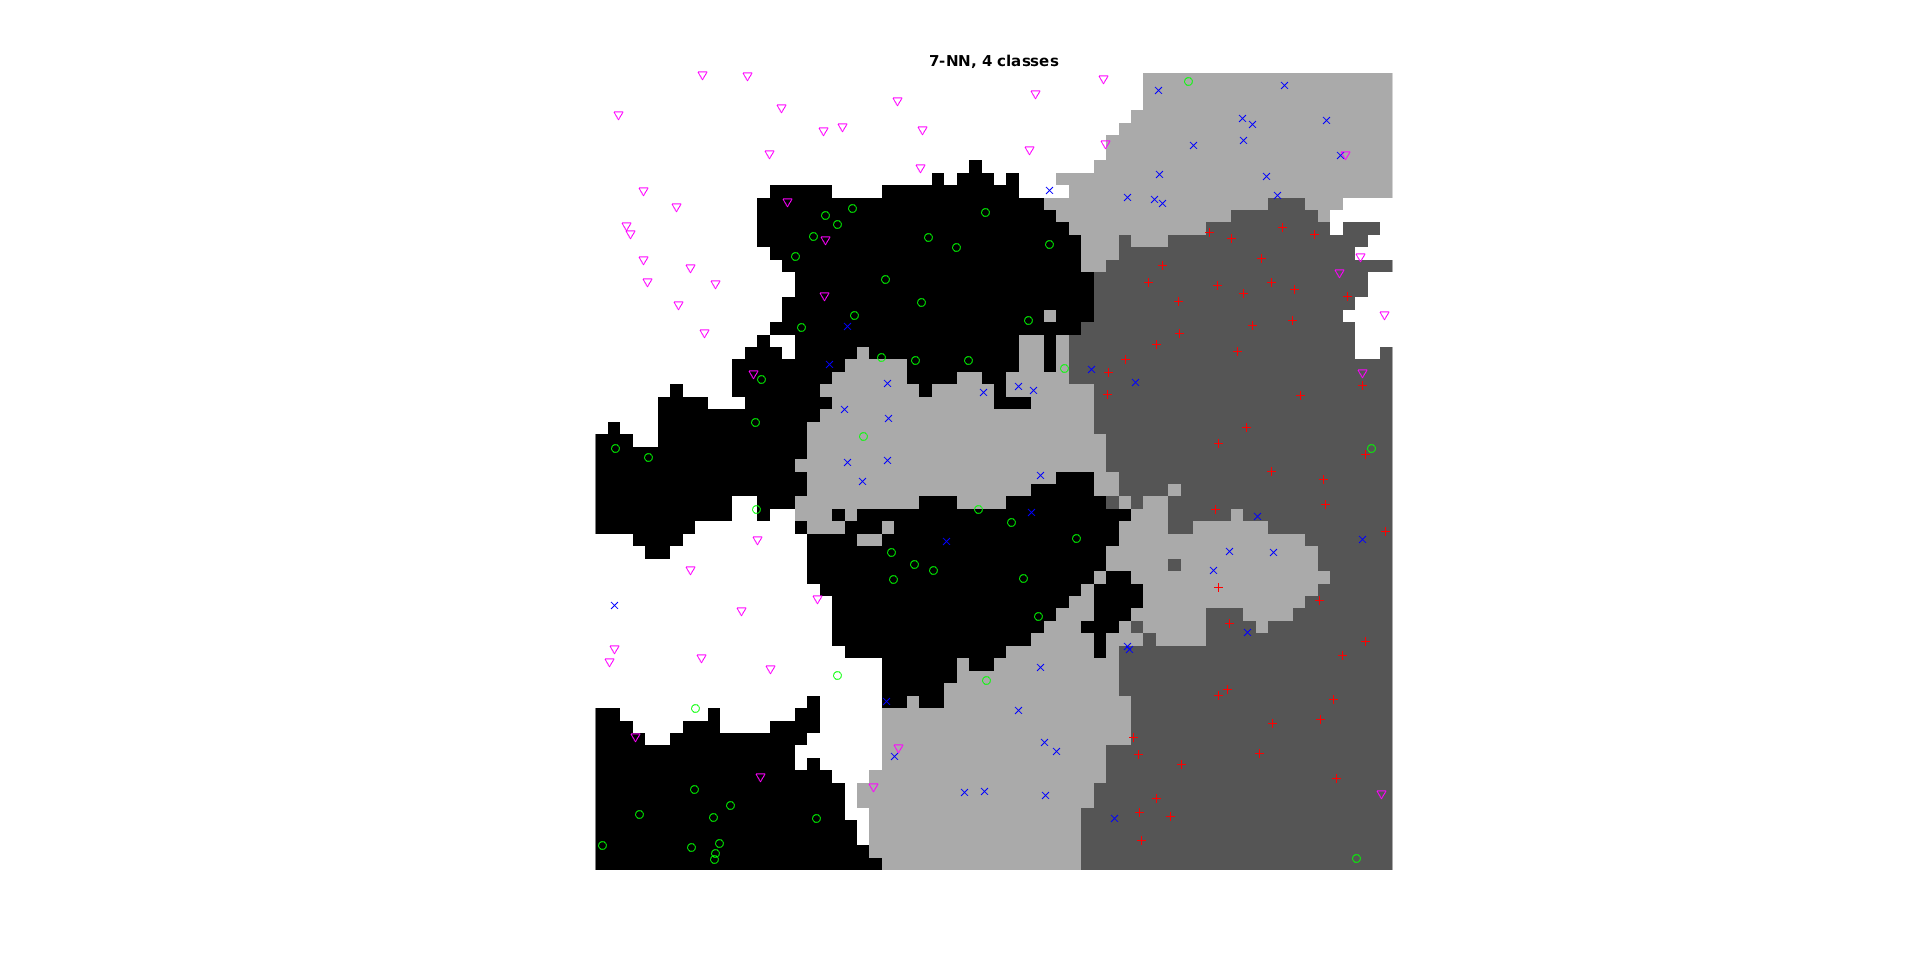
\includegraphics[width=.8\textwidth]{assign2_4_7.png}
    \caption{Classification grid of the data set using KNN (for $k=7$)}
    \label{fig2.4d}
  \end{subfigure}
  \caption{Classification grids for different $k$s}
  \label{fig2.4_a}
\end{figure}

\begin{figure}[H]
 \centering
 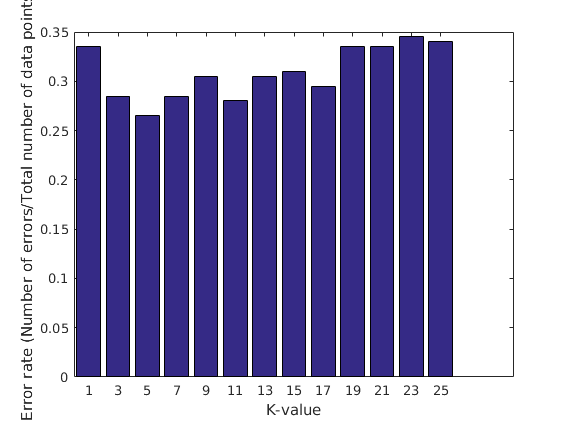
\includegraphics[width=.7\textwidth]{assign2_4_b.png}
 \caption{Error rate for different values of $k$ using leave-one-out cross validation.}
 \label{fig2.4_b}
\end{figure}

\section{Parzen windows, posterior probabilities}
\subsection{}
We computed the following densities using the code given in the appendix:
% \begin{array}
% 
% \end{array}


\section*{Appendix}
\lstinputlisting{../Code/assign1_1.m}
\lstinputlisting{../Code/assign1_2.m}
\lstinputlisting{../Code/KNN.m}
\lstinputlisting{../Code/assign2_3.m}
\lstinputlisting{../Code/assign3_1.m}

\end{document}
